
\documentclass[11pt]{exam} % https://www.ctan.org/pkg/exam?lang=en

\usepackage[lmargin=1.in,rmargin=1.in,tmargin=1.in,bmargin=1in]{geometry}
\usepackage{setspace}
\usepackage[pdftex]{graphicx}
\usepackage{titling}
\usepackage[
	pdfauthor={Brian Weinstein},
	pdftitle={Homework 2},
	bookmarks=true,
	colorlinks=true,
	linkcolor=blue,
	urlcolor=blue,
	citecolor=blue,
	pdftex,
	linktocpage=true
	]{hyperref}
\usepackage[textsize=tiny]{todonotes}
\usepackage{float}
\setlength\parindent{0pt}


\qformat{\textbf{Question \thequestion: \thequestiontitle}\quad \hfill}


\pagestyle{headandfoot}
\runningheadrule
\firstpageheader{}{}{}
\runningheader{\thetitle}{\theauthor}{\thedate}
\firstpagefooter{}{}{}
\runningfooter{}{}{}





\usepackage{xcolor}
\usepackage{adjustbox}
\usepackage{verbatim}
\definecolor{shadecolor}{rgb}{.9, .9, .9}

\newenvironment{code}%
   {\par\noindent\adjustbox{margin=1ex,bgcolor=shadecolor,margin=0ex \medskipamount}\bgroup\minipage\linewidth\verbatim}%
   {\endverbatim\endminipage\egroup}





\begin{document}


\title{STAT S4240 002, Homework 2}
\author{Brian Weinstein (bmw2148)}
\date{July 23, 2015}
\maketitle



\begin{questions}



\titledquestion{PCA}

\begin{parts}



\part Column means
\begin{code}
> apply(rawData, 2, mean)
       x1        x2        x3        x4        x5 
 6.049104 -8.277221  4.665532  7.914270 62.138753 
\end{code}
 
Row means
\begin{code}
> apply(rawData, 1, mean)
  [1]  -0.1277116  20.8162864  -8.8984358  25.5999204  -9.7472153
  [6]  64.0626702  22.0392371  23.3914888  31.7598224 -13.8680290
...
 [91]   1.2105932  21.2145724  -8.4896595  19.0639963  20.9767512
 [96]   3.5962333  22.3461063   0.7145014   6.3080005  64.8829556
\end{code}

The nonzero column means indicate that each variable isn't centered. In this context the row means indicate \todo{row means?}. 
 
 
\part Empirical covariance matrix
\begin{code}
          x1         x2        x3        x4        x5
x1  72.96417  -83.90858  53.23708  120.1162  568.4105
x2 -83.90858  110.89101 -63.89570 -115.9430 -817.3388
x3  53.23708  -63.89570  39.60282   83.7386  445.2511
x4 120.11620 -115.94304  83.73860  232.1333  683.5587
x5 568.41046 -817.33884 445.25112  683.5587 6288.8569
\end{code}

The diagonal values tell us the variance of the variable indicated in the column (or equivalently, the row). The off-diagonal elements indicate the covariance between the two variables that intersect at that element.

\part The eigenvalues and eigenvectors of the empirical covariance matrix \texttt{sig}
\begin{code}
> eigen(sig)
$values
[1] 6.557348e+03 1.868951e+02 2.038354e-01 9.775594e-04 9.373658e-05

$vectors
            [,1]       [,2]         [,3]        [,4]        [,5]
[1,]  0.09009603 -0.3247102 -0.383470773  0.82286709  0.24957150
[2,] -0.12797842  0.1364755  0.227047683 -0.11412319  0.94890526
[3,]  0.07028767 -0.1941349  0.894987159  0.37278501 -0.13191135
[4,]  0.11077853 -0.9008231 -0.019718518 -0.40719485  0.10024632
[5,]  0.97892389  0.1636064  0.002946326 -0.07133967  0.09921159
\end{code}

Since it's a symmetric matrix, \texttt{sig} has the same left eigenvectors as right eigenvectors.

\part The loadings are the eigenvectors (see part c). The scores are:
\begin{code}
> data%*%evecs
              [,1]        [,2]         [,3]          [,4]          [,5]
  [1,]  -58.606720   6.8128841  0.358690823 -0.0080251123  6.008437e-03
  [2,]   17.967890 -10.0253314  0.313590316 -0.0051005161 -1.454011e-02
  [3,] -103.557582   0.7721199  0.080912663  0.0422848507  5.511172e-04
...
 [98,]  -47.475844  14.1883799  0.376152574 -0.0311565338 -9.890383e-03
 [99,]  -35.054501   1.1602437 -0.421041558 -0.0220654373  5.471521e-04
[100,]  209.221180 -15.3655377 -0.100374179  0.0323254561  4.388429e-03
\end{code}

\part

asdf













\end{parts}

\titledquestion{question}


\titledquestion{\href{http://www-bcf.usc.edu/~gareth/ISL/}{James} 3.7.3}


\begin{parts}
\part
asdfasdf
\end{parts}


%\begin{figure}[H]
%	\centering
%	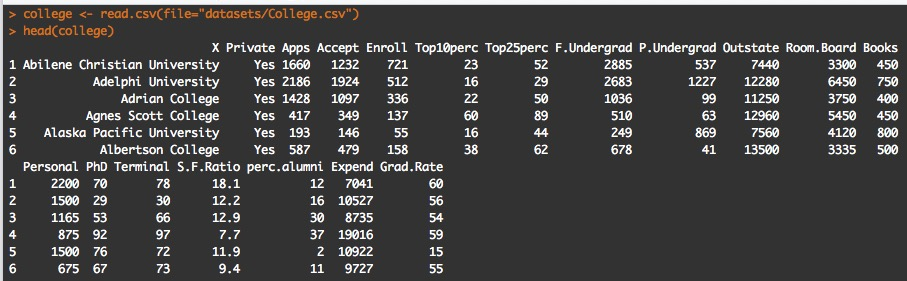
\includegraphics[width=6.5in]{8a.jpeg}
%	%\caption{}
%	%\label{fig:figName}
%\end{figure}


\end{questions}

\listoftodos

\end{document}